################# this file is just for paragraphs that I excluded but might want to access later on ###################

\subsubsection{Phasing bias / switch errors}

{\color{red}[AS WITH THIS SECTION IN GENERAL, THERE ARE TWO ISSUES HERE: (1) PHASING ERRORS, WHICH WILL ADD (RANDOM) NOISE AND (2) PHASING BIAS, WHICH WILL BIAS ADNA SAMPLES TO LOOK MORE LIKE THE REFERENCE. I'M NOT SURE THIS SECTION SHEDS MUCH LIGHT ON THIS. PERHAPS IT'S BETTER TO TRY THIS IN POBI -- HAVE YOU IMPUTED (LOW DENSITY) POBI USING 1KGP? THAT WOULD BE GOOD TO DO, AS IT MAY BIAS CORNWALL TO LOOK MORE LIKE DEVON DUE THEM BOTH STARTING TO LOOK MORE LIKE 1KGP BRITISH. ONE COMPLICATION HERE THOUGH IS THAT 1KGP BRITISH CONTAIN CORNWALL INDS, SO I THINK YOU NEED TO PROBABLY REMOVE GBR FROM THE REFERENCE.]}Phasing relies on having a reference panel of individuals from whom it is possible to reconstruct the the haplotypes of a target individual from. A 'switch-error' occurs when an individual incorrectly switches from copying from the correct to an incorrect reference haplotype, or in effect false recombination events which occur between the inferred haplotypes compared with the true haplotypes \cite{choi2018comparison}. Previous research has shown that reduced coverage results in an increase in the number of switch errors, presumably because of the increased chance of incorrectly called genotypes at lower coverage \cite{rubinacci2021efficient}. Therefore, one potential cause of low coverage samples moving towards the origin of the PCA could be an increase in switch errors caused by an increase in genotyping errors. For example, a switch error may arise when a true heterozygous position is incorrectly called as a homozygous position due to low coverage, and the correct allele on one of the haplotypes cannot be phased. 

The possible effect of increased switch errors at lower coverage can be testing by running ChromoPainter under the unlinked model, which assumes a model of linkage equilibrium between neighbouring SNPs and essentially regresses to a model of allele frequency differences \cite{Lawson2012}. Thus, switch errors / incorrectly phased heterozygous positions would not be expected to influence the painting under the unlinked model. To test the potential effect of phasing  bias / switch errors, I performed the same painting as in Fig. \ref{fig:PCA_panel_allInds_unlinked.allCoverage}, but in unlinked mode. 

\subsection{Imputation bias}

The previous section indicated that phasing issues are {\color{red}not} the primary cause of {\color{red}coverage-related bias[STILL NOT CLEAR WE'VE SHOWN IT'S BIAS]}.

One other possible cause could be the tendency to incorrectly assign genotypes as homozygous when they are in fact heterozygous. This is because when a true heterozygous genotype is covered by a low number (e.g.\ 1 or 2) reads, there is a higher probability that there are no reads sampling one of the alleles. {\color{red}[THIS ISN'T RIGHT -- IF COVERED BY A SINGLE READ, THERE IS A 100\% CHANCE ONE OF THE ALLELES IS NOT SAMPLED; I THINK YOU MEAN IF A POSITION IS COVERED BY TWO READS?]For example, if we assume that there is an equal probability of a read sampling either allele, then if the position is only covered by a single read, there is a 50\% chance one of the alleles would not be sampled and the genotype would be incorrectly assigned as a homozygous.} Even when there are 5 reads covering a position, there is still 3.125\% chance that one of the alleles would not be sampled by a read. Because homozygous genotypes do not need to be phased, these errors would not be mitigated by running ChromoPainter in unlinked mode.

\subsection{Explicit test of cause}

To test the explicit cause of the coverage-related bias, I removed different sets of SNPs from downsampled individuals. I took the phased haplotypes for all 5 individuals downsampled to 0.1x and 0.5x and compared them to the same individuals at full coverage. Positions were classified as different kinds of mismatch between the downsampled and full coverage individual; a) dosage mismatch if the dosage differed, b) 'hap-A' mismatch if the alleles on the first haplotype differed, c) 'hap-B' mismatch if the alleles on the second haplotype differed and d) 'hap-a-hap-b' mismatch if the alleles on the first and second haplotypes differed.{\color{red}[I COULDN'T FOLLOW THIS SECTION -- E.G. HOW DO YOU ASSIGN A ``HAPLOTYPE''?]}

NB: I am waiting for this to finish so don't have the results yet.


\begin{figure}[htp]
    \centering
    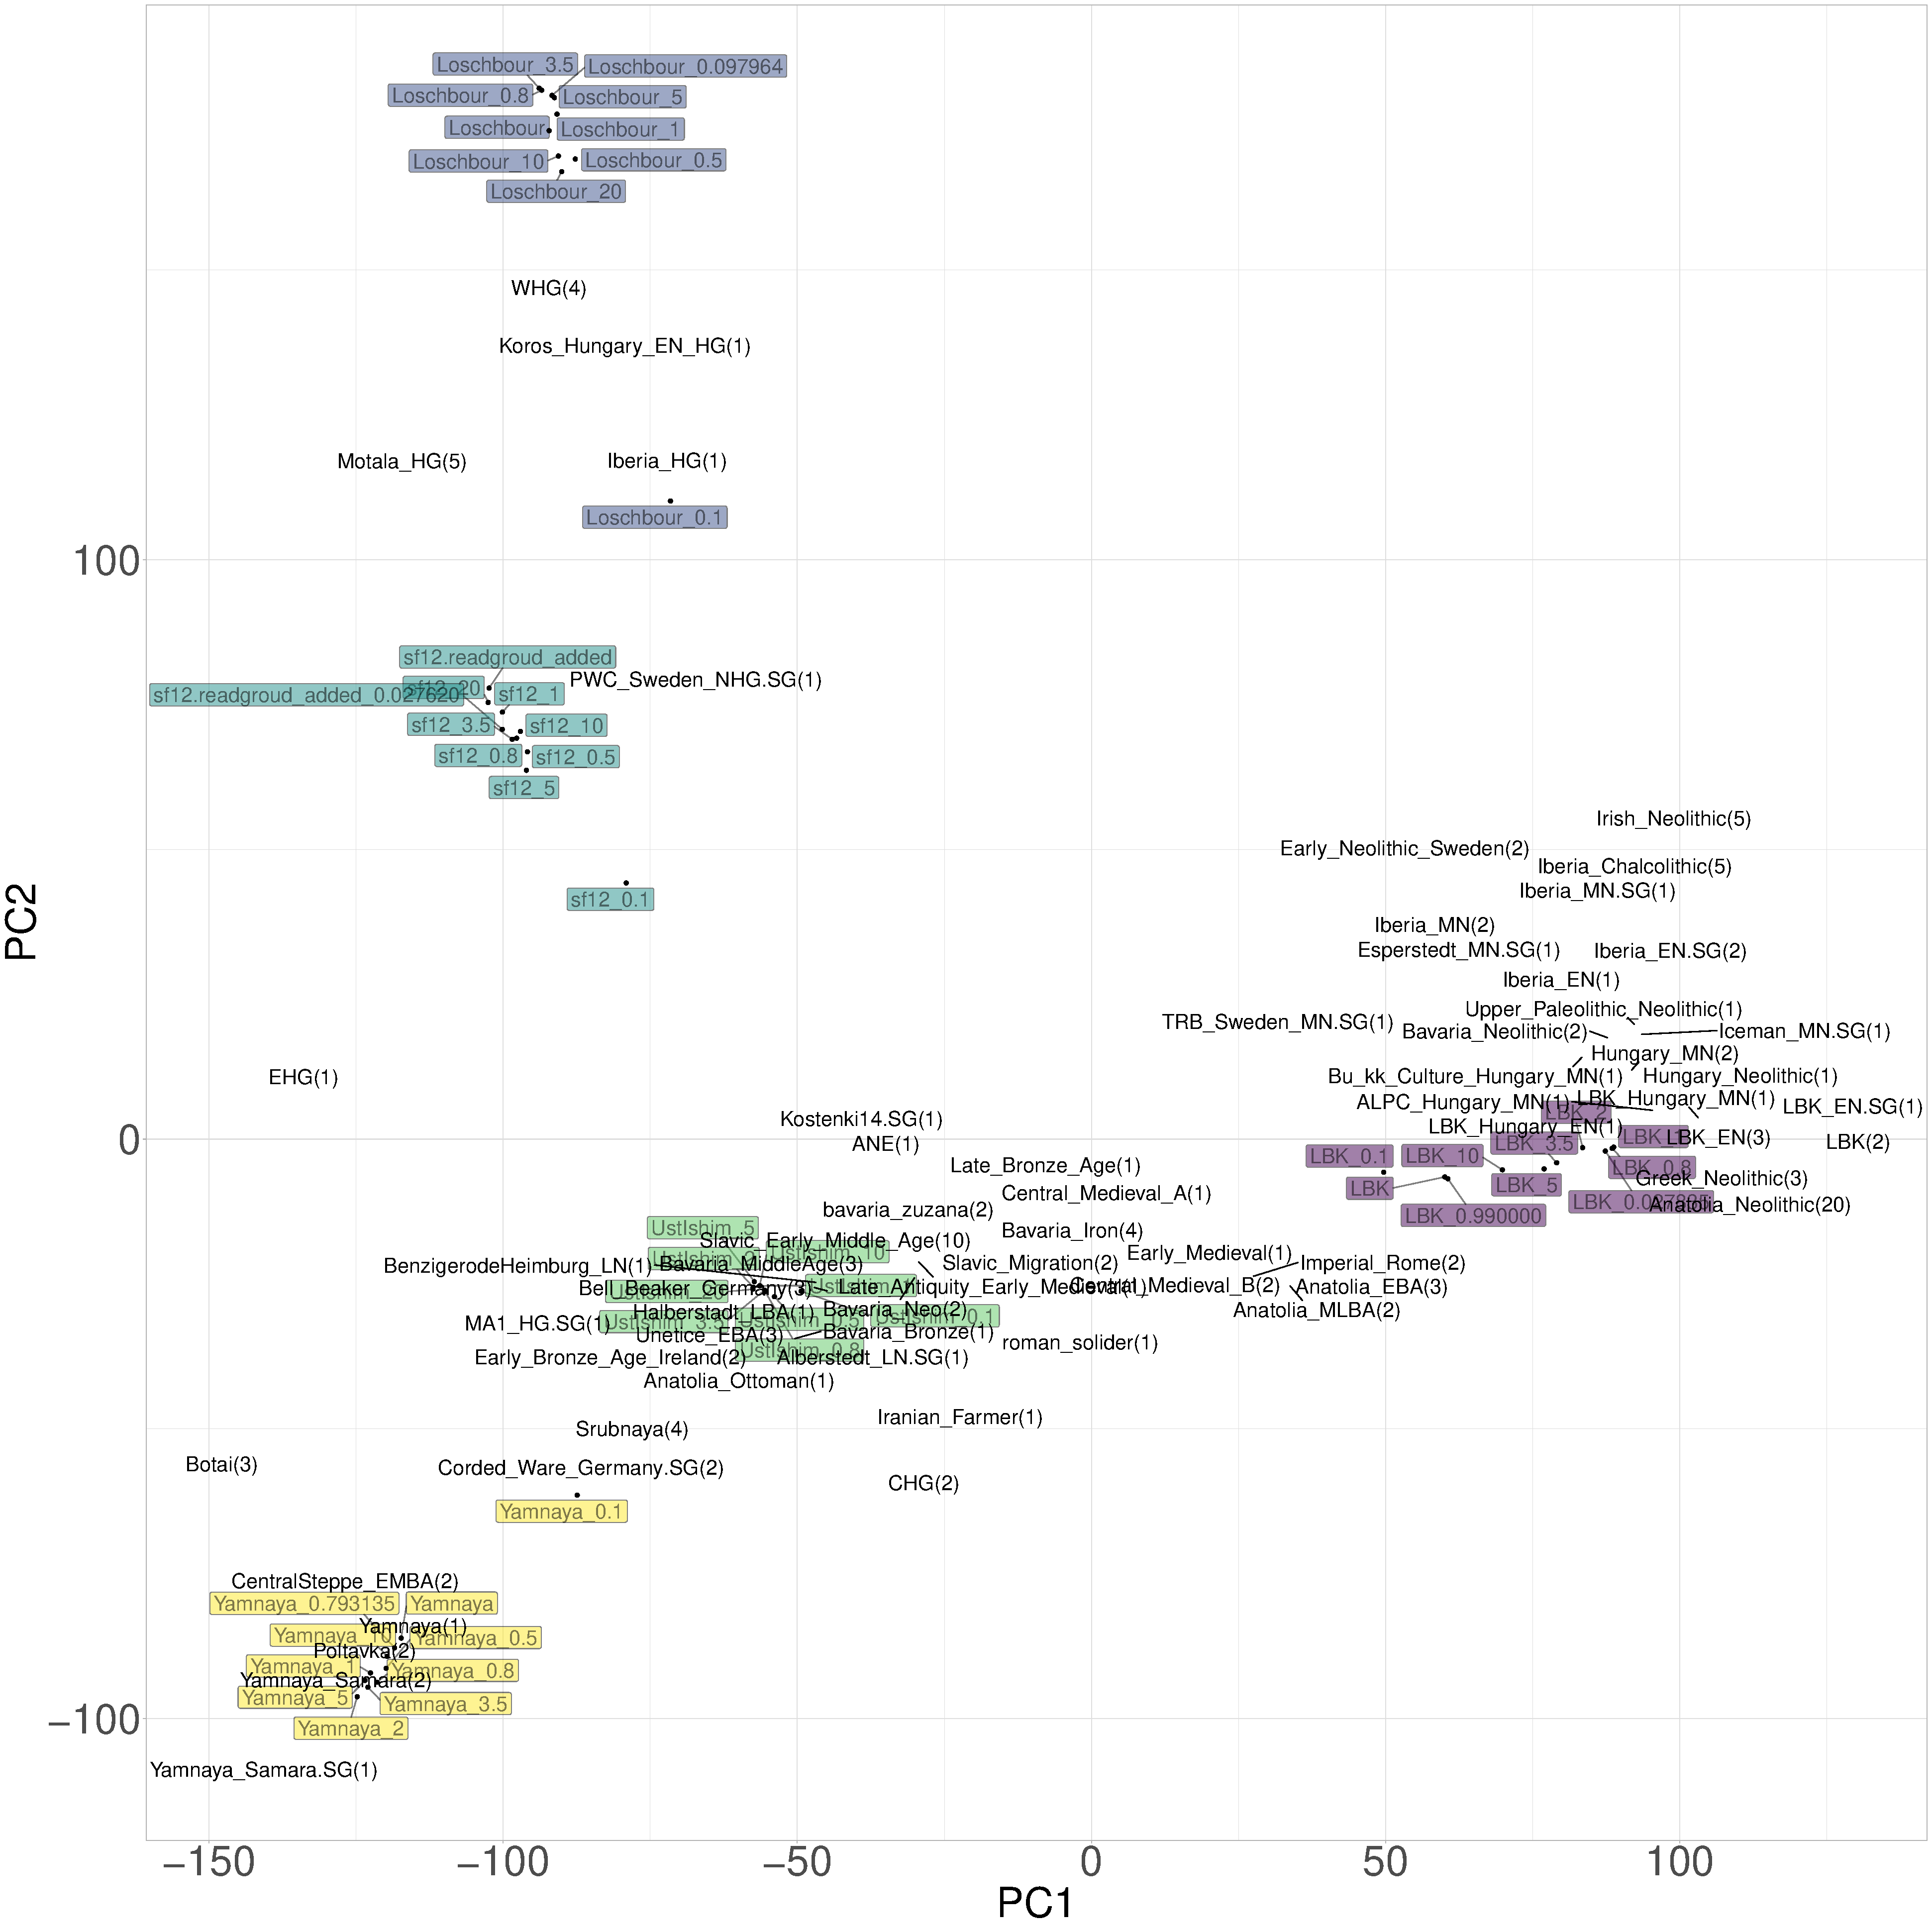
\includegraphics[width=1.0\textwidth]{../images/chapter1/PCA_panel_allInds_unlinked.allCoverage.pdf}
    \caption{Principle component analysis (PCA) of downsampled, full coverage and reference ancient individuals generated from the unlinked chunklengths matrix. Full coverage and downsampled genomes of the same individual are coloured the same. Reference individuals are grouped into populations plotted as the mean principle components for all individuals within the population.}
    \label{fig:PCA_panel_allInds_unlinked.allCoverage}
\end{figure}

Fig. \ref{fig:PCA_panel_allInds_unlinked.allCoverage} shows the same PCA, but on the chunkcounts matrix from the corresponding unlinked painting (because 'chunks' are formed from linked SNPs, there is no lengths matrix output from the unlinked model - the equivalent is the counts matrix). It is clear that the same issue persists and that lower coverage individuals are still pulled towards the centre of the PCA, suggesting that phasing switch errors are not the main issue. It is also clear that much of the population structure (e.g. the ability to separate the Neolithic and Bronze Age clusters) disappears when using the unlinked painting.


